{

\setlength{\parindent}{0pt}
\setlength{\parskip}{1em}

\chapter{Preliminaries}

\section{Cloud Segmentation in Satellite Imagery}

The first successful weather satellite, TIROS-1, was launched on April 1, 1960.
During its mission it returned thousands of photographs showing cloud-cover views of the Earth,
which proved extremely helpful for predicting large-scale weather changes and significantly improving forecasting capabilities.

From this point, the need to distinguish cloud from non-cloud regions became clear, either to remove clouds for
surface-focused analyses or to study the cloud field itself, both of which require separating clouds from the rest of the image.
In time-series for weather forecasting, the motion of cloud layers can be tracked and predicted by expert analysts.
Automating this process is one precise example where cloud segmentation is essential.

Early segmenation workflows relied on manual inspection and empirical thresholding.
Over the years, these evolved into image processing methods, then classical machine learning,
and today into deep learning models, most notably \glspl{cnn}, to achieve reliable, scalable cloud segmentation.

Automated extraction of cloud masks can be challenging when analyzing only the visible light bands: \gls{rgb}.
With additional sensors, satellites capture other wavelengths such as \glsxtrlong{nir}, Shortwave Infrared, and Thermal Infrared.
Each of these channels can benefit cloud segmentation in its own way.
Given the 38-Cloud dataset, which contains \gls{rgb} and \gls{nir} channel images from the Landsat 8 mission, this work will focus on them.
\gls{nir} is especially helpful for distinguishing clouds over liquid water, where it is strongly absorbed.
It also helps separate clouds from green vegetation, which is bright in the \gls{nir} band.

However, the OOV-CUBE satellite hosts only an \gls{rgb} camera onboard.
Cloud segmentation utilizing only these channels is possible, but may yield less accurate masks.
Therefore, the necessity to provide and evaluate a model that uses only the visible channels will be considered in this work.

\clearpage
\section{Convolutional Neural Networks for Cloud Segmentation}
\label{subsec:stateoftheart}

\glspl{cnn} are a class of neural networks that apply small, learnable filters (convolutional kernels)
across an image to extract spatial features. A \gls{cnn} typically consists of multiple convolutional layers stacked sequentially.
Each layer applies a set of filters that capture different visual patterns, such as edges, textures, or simple shapes.
As the network goes deeper, the spatial resolution of the image decreases, while the depth (number of channels) increases.
This is a result of applying multiple filters and optionally using pooling layers,
which downsample feature maps to reduce computational complexity and introduce spatial invariance.

In classical image processing, filter parameters can be hand-crafted to extract specific features. %(for example, Sobel or Laplacian operators).
In deep learning, however, these parameters are learned from data.
Given a sufficiently deep network of filters, gradient descent techniques are applied to a loss function
that measures the discrepancy between the network's output and the known \gls{gt}.
In this way, the network is optimized to extract the necessary information from images.

In image segmentation tasks such as cloud detection, preserving spatial resolution is critical.
Therefore, architectures often include an upsampling mechanism to reconstruct high-resolution output from compressed feature representations.
This is achieved through transposed convolution (also known as deconvolution).
While standard convolution reduces spatial resolution by aggregating local pixel values, transposed convolution performs the reverse:
it distributes each value in the smaller feature map across a larger output, effectively increasing spatial dimensions and reversing the compression.

One of the most influential architectures for image segmentation is the \code{U-Net}.
Originally introduced by Ronneberger et al.~\cite{ronneberger2015u} for biomedical image segmentation,
\code{U-Net} has become a standard in many domains, including remote sensing and cloud detection.
This architecture has proven highly effective for segmentation tasks, even with limited training data.
A \code{U-Net} consists of an encoder-decoder structure.
The encoder compresses the input image spatially while increasing its feature dimensionality.
The decoder then reconstructs the spatial dimensions, progressively reducing the number of channels.
This yields an output image with the same spatial dimensions (height and width) as the input, but could have a various number of channels, depending on the perceived task.
The \code{U-Net} architecture shown in \autoref{fig:unet-architecture} was used by Mohajerani et al.~\cite{CloudNet2019} for their cloud detection algorithm.

A key innovation in \code{U-Net} is the use of residual (skip) connections \cite{he2015deepresiduallearningimage},
which directly link feature maps from the encoder to corresponding layers in the decoder with the same spatial size.
These connections preserve fine-grained spatial details and significantly enhance segmentation quality.
Moreover, they mitigate the vanishing gradient problem, facilitating the training of deeper networks and improving convergence.

\begin{figure}[H]
  \centering
  \includegraphics[width=\textwidth]{files/U-Net_cloud_detection1.png}
  \caption{U-Net architecture adapted for cloud detection by Mohajerani et al.~\cite{CloudNet2019}}
  \label{fig:unet-architecture}
\end{figure}

\section{Evaluation Metrics for Cloud Segmentation}
\label{subsec:evalmetrics}

After performing a binary cloud segmentation task, a \gls{cnn} outputs a probability mask
with continuous values in \([0,1]\).
A threshold is then selected to binarize the probability mask:
values at or above the threshold are set to one (cloud present), and values below the threshold are set to zero (no cloud present).


The predicted cloud mask is then compared with the \gls{gt} mask.
For each overlapping pixel, four outcomes are possible:

\begin{itemize}
    \item \textbf{True Positive (TP):} Pixel is cloud in the prediction and in the \gls{gt}.
    \item \textbf{True Negative (TN):} Pixel is not cloud in the prediction and in the \gls{gt}.
    \item \textbf{False Positive (FP):} Pixel is cloud in the prediction but not in the \gls{gt}.
    \item \textbf{False Negative (FN):} Pixel is not cloud in the prediction but cloud in the \gls{gt}.
\end{itemize}

Using these outcomes, widely accepted metrics for evaluating \gls{cnn} performance on the cloud segmentation task are defined.
The following metrics will be used in this work:

\[
\begin{array}{llcl}
\text{Accuracy}  &= \dfrac{TP + TN}{TP + TN + FP + FN} 
& \quad \text{Precision} &= \dfrac{TP}{TP + FP} \\[1.2em]
\text{Recall}    &= \dfrac{TP}{TP + FN} 
& \quad \text{Jaccard Index (IoU)} &= \dfrac{TP}{TP + FP + FN} \\[1.2em]
\text{Dice Coefficient} &= \dfrac{2TP}{2TP + FP + FN} & &
\end{array}
\]

Accuracy represents the fraction of correctly predicted pixels relative to the total number of pixels.
Precision reflects how selective the model is: high precision means the model labels a pixel as cloud only when confident,
which may increase false negatives (missed clouds).
High recall, on the other hand, indicates the model tries to catch as many clouds as possible, which may increase false positives.
The Jaccard Index (Intersection over Union) \cite{jaccardindex} and the Dice Coefficient \cite{dicecoefficient}
both relate precision and recall and measure the overlap between the predicted and \gls{gt} sets.

Note that the optimal threshold, the value that yields the closest match between the predicted binary mask and the \gls{gt}, is not necessarily \(0.5\).
It can lie anywhere in \([0,1]\). A common approach is to evaluate the precision-recall curve and select the threshold according to a chosen criterion (for example, maximum F1-Score) \cite{prc, f1}.


\section{38-Cloud dataset}
\label{subsec:dataset}

Landsat 8\footnote{\url{https://landsat.gsfc.nasa.gov/satellites/landsat-8/}} is an Earth observation satellite launched on February 11, 2013,
providing high-resolution multispectral imagery, including \gls{rgb}, \gls{nir}, and Thermal Infrared bands.
This thesis utilizes a dataset consisting of 38 annotated satellite images from the Landsat 8 mission,
commonly referred to as the 38-Cloud dataset\footnote{\url{https://github.com/SorourMo/38-Cloud-A-Cloud-Segmentation-Dataset}}.
It has been introduced and adapted in the following scientific publications \cite{CloudDet2018, CloudNet2019}.
38 images are divided into a training set containing 18 scenes and a test set with the remaining 20 scenes.
The folder structure of the dataset is illustrated in \autoref{fig:dsFolderStruct}.

Each image consists of four spectral channels: \gls{rgb} and \gls{nir}, along with a manually annotated \gls{gt} mask that labels cloud regions at the pixel level.
The four spectral channels are encoded using \glspl{uint16} per pixel, whereas the \gls{gt} masks are represented with \glspl{uint8}.
A single raw image at full resolution of approximately \ensuremath{8000\times8000} pixels would result in a file size of around 1GB.
Moreover, processing such images would require model input tensors of shape \ensuremath{batchsize\times8000\times8000\times4} in \gls{float32} after normalization.
Since efficient training typically necessitates a \ensuremath{batchsize} greater than one,
this setup would impose substantial computational demands due to increased model size and would significantly slow down both training and inference ---
making it particularly unsuitable for deployment on embedded systems.
To address this, the dataset is provided in a pre-cropped format, with each image and its corresponding \gls{gt} mask divided into \ensuremath{384\times384} pixel patches.
These patches are saved as \code{.TIF} files within their respective channel-specific directories, such as \code{train\_red}, \code{train\_green}, and so forth.
The \gls{gt} patches for training are stored in the \code{train\_gt} directory.

It is important to note, however, that pre-cropped \gls{gt} patches are not available for the test subset.
Instead, complete scene \gls{gt} masks are provided in the \code{Entire\_scene\_gts} directories for both the train and test subsets.

\begin{figure}[!h]
\dirtree{%
.1 38-Cloud Dataset.
.2 38-Cloud\_training.
.3 train\_red.
.3 train\_green.
.3 train\_blue.
.3 train\_nir.
.3 train\_gt.
.3 Natural\_False\_Color.
.3 Entire\_scene\_gts.
.3 training\_patches\_38-Cloud.csv.
.3 training\_sceneids\_38-Cloud.csv.
.2 38-Cloud\_test.
.3 test\_red.
.3 test\_green.
.3 test\_blue.
.3 test\_nir.
.3 Natural\_False\_Color.
.3 Entire\_scene\_gts.
.3 test\_patches\_38-Cloud.csv.
.3 test\_sceneids\_38-Cloud.csv.
.2 training\_patches\_38-cloud\_nonempty.csv.
}
\caption{Folder structure of the 38-Cloud dataset.}
\label{fig:dsFolderStruct}
\end{figure}

The examples of training patches from all four spectral channels and the corresponding \gls{gt} mask at a fixed location
are shown in \autoref{fig:patch_example} as normalized greyscale images. 

\begin{figure}[!h]
  \centering
  \begin{subfigure}[t]{0.19\textwidth}
    \includegraphics[width=\linewidth]{files/examples/red_patch.png}
    \caption{Red}
  \end{subfigure}
  \hfill
  \begin{subfigure}[t]{0.19\textwidth}
    \includegraphics[width=\linewidth]{files/examples/green_patch.png}
    \caption{Green}
  \end{subfigure}
  \hfill
  \begin{subfigure}[t]{0.19\textwidth}
    \includegraphics[width=\linewidth]{files/examples/blue_patch.png}
    \caption{Blue}
  \end{subfigure}
  \hfill
  \begin{subfigure}[t]{0.19\textwidth}
    \includegraphics[width=\linewidth]{files/examples/nir_patch.png}
    \caption{NIR}
  \end{subfigure}

  \vspace{0.5em}

  \begin{subfigure}[t]{0.19\textwidth}
    \includegraphics[width=\linewidth]{files/examples/gt_patch.png}
    \caption{\gls{gt}}
  \end{subfigure}

  \caption{Four spectral input patches and the corresponding \gls{gt} mask.}
  \label{fig:patch_example}
\end{figure}

Each \gls{rgb}, \gls{nir}, and \gls{gt} patch follows a unified filename convention:

\begin{lstlisting}
<band>_patch_<index>_<row>_by_<col>_<metadata>.TIF
\end{lstlisting}

The corresponding components are:

\begin{tabularx}{0.97\textwidth}{@{\hspace{\parindent}}>{\ttfamily}p{2.7cm}@{\hspace{0.3em}}L}
\textbf{band} \dotfill & Indicates the spectral band or \gls{gt} mask. \\
\textbf{index} \dotfill & Ordinal number of the patch within the scene. Patches are extracted sequentionally from left to right, top to bottom. \\
\textbf{row \& col} \dotfill & Patch's position in the scene, specified by its row and column indices. \\
\textbf{metadata} \dotfill & Encodes the satellite and sensor ID, preprocessing precision, scene path/row, acquisition and processing dates, and collection tier metadata. \\
\end{tabularx}

An example filename:

\begin{lstlisting}
blue_patch_103_5_by_11_LC08_L1TP_063013_20160920_20170221_01_T1.TIF
\end{lstlisting}

This naming scheme ensures consistency and supports automated patch retrieval across channels.
The filenames, excluding the \code{band} prefix, are listed in the \code{training\_patches\_38-Cloud.csv} and \code{test\_patches\_38-Cloud.csv} files, respectively.
The corresponding scene-level filenames are stored in \code{training\_sceneids\_38-Cloud.csv} and \code{test\_sceneids\_38-Cloud.csv}.

One notable detail is that, due to the cropping and padding of border patches (to standardise the patch size to \ensuremath{384\times384} pixels) and the tilted geometry of Landsat 8 imagery,
some resulting patches contain no meaningful information --- appearing completely black with all-zero pixel values across all four channels.
These zero-information patches were excluded from the training and validation sets to avoid overrepresenting non-informative inputs,
which could degrade the model's ability to learn meaningful patterns.
The remaining useful patch names are stored in \code{training\_patches\_38-cloud\_nonempty.csv} file.

Together, these \code{.csv} files serve as the basis for dataset construction in \secshortref{sec:data}.
Furthermore, the attributes such as \code{index}, \code{row \& col} will be directly utilized during the stitching process described in \secshortref{subsec:testing}.

For visualization purposes, the full scene images are rendered using a false-color composite.
However, these visualizations were not used as input for the \gls{cnn} during training, validation, or inference.
They served solely as visual references for qualitative inspection by the human observer.
The corresponding images are located in the \code{Natural\_False\_Color} directories.
An example scene is shown below in \autoref{fig:false_color_scene}: 

\begin{figure}[H]
  \centering
  \includegraphics[width=0.7\textwidth]{files/examples/scene.jpg}
  \caption{False-color composite of an entire scene.}
  \label{fig:false_color_scene}
\end{figure}


\section{Quantization Concept}
\label{subsec:quantization}

Quantization is a mathematical method that maps a large set of (typically continuous) values to a smaller, discrete and countable set.
Its first practical application can be traced back to 1957, in the context of pulse-code modulation within the field of signal processing.
The earliest formal scientific documentation of the method appears in a publication from 1982,
which is based on a draft manuscript originally authored in 1957 \cite{firstQuantization}.

This technique is now widely employed in machine learning \cite{MLQuantization1, MLQuantization2, quantnnwhite}.
Quantization significantly reduces model size \cite{quantcompression} by compressing numerical precision, typically at the cost of a controlled reduction in accuracy.
Two primary quantization methods are commonly used: general asymmetric zero-point quantization, and its special case ---
symmetric absolute maximum (absmax) quantization.
In the context of this work, the general asymetric approach is of primary importance.

To perform quantization, the boundaries \( x_{\text{min}} \) and \( x_{\text{max}} \) of the original (floating-point) range,
and \( q_{\text{min}} \) and \( q_{\text{max}} \) of the target (quantized) value set must be defined.
Once these are known, the corresponding scale and zero-point parameters are computed according to the following equations:

\clearpage
\begingroup
\setlength{\jot}{8pt} % tighten spacing between lines (default ≈3pt)
\begin{align}
\text{scale} &= \frac{x_{\text{max}} - x_{\text{min}}}{q_{\text{max}} - q_{\text{min}}} \label{eq:scale}\\[-2pt]
\text{zero-point} &= \operatorname{round}\!\left( q_{\text{min}} - \frac{x_{\text{min}}}{\text{scale}} \right) \label{eq:zeropoint}
\end{align}
\endgroup

With these parameters determined,
input value \( x \) can be transformed into quantized form \( q_{\text{x}} \) and subsequently dequantized to an approximate value \( x_{\text{q}} \) using the following formulas:

\begingroup
\setlength{\jot}{8pt} % line spacing inside align (default ~3pt)
\begin{align}
q_{\text{x}} &= \operatorname{round}\!\left(\frac{x}{\text{scale}}\right) + \text{zero-point} \label{eq:quantize}\\[-2pt]
x_{\text{q}} &\approx \left( q_{\text{x}} - \text{zero-point} \right)\cdot \text{scale} \label{eq:dequantize}
\end{align}
\endgroup

It is essential to note that both the scale and zero-point must be preserved in order to carry out the quantization and dequantization processes.
For every value range subject to quantization, a unique pair of these parameters exists.

The following example demonstrates the use of zero-point quantization. Consider a set of continuous values ranging from -9.75 to 3.00.
To map this range onto a discrete set defined by the integer interval [-128, 127], the scale and zero-point are calculated using \autoref{eq:scale} and \autoref{eq:zeropoint}:

\[
\begin{array}{rlrl}
\text{scale} &= \dfrac{3.00 - (-9.75)}{127 - (-128)} = 0.05
& \quad
\text{zero-point} &= \text{round}\!\left(-128 - \dfrac{-9.75}{\text{scale}}\right) = 67
\end{array}
\]

After this step, every value from the original dataset can be represented by its corresponding quantized counterpart.
The following calculations illustrate the quantization and subsequent dequantization of four examples using \autoref{eq:quantize} and \autoref{eq:dequantize}:
\( x = 0 \), \( x = 3.00 \), \( x = 2.98 \), \( x = 2.95 \):

\[
\begin{array}{rlrl}
q_{0}     &= \text{round}\!\left(\tfrac{0}{0.05} \right) + 67 = 67
& x_{67}   &\approx (67 - 67)\cdot 0.05 = 0 \\[0.5ex]
q_{3.00}  &= \text{round}\!\left(\tfrac{3.00}{0.05} \right) + 67 = 127
& x_{127} &\approx (127 - 67)\cdot 0.05 = 3.00 \\[0.5ex]
q_{2.98}  &= \text{round}\!\left(\tfrac{2.98}{0.05} \right) + 67 = 127
& x_{127} &\approx (127 - 67)\cdot 0.05 = 3.00 \\[0.5ex]
q_{2.95}  &= \text{round}\!\left(\tfrac{2.95}{0.05} \right) + 67 = 126
& x_{126} &\approx (126 - 67)\cdot 0.05 = 2.95
\end{array}
\]


The last three examples illustrate the precision loss introduced by quantization.
In this case, any input between 2.925 and 3.00 (depending on the rounding convention) is mapped,
after conversion, to one of two discrete values: 126 or 127.


It is important to emphasize that the scale parameter etirely defines the quantizer's precision,
under the assumption that the bit-width (256 discrete representable values in this case) is fixed,
as well as the floating-point range from -9.75 to 3.00 being evenly distributed across the entire interval and free of outliers.

In practice, more advanced quantization techniques may be employed, such as outlier-aware clipping, per-axis and per-tensor quantization,
symmetric and asymmetric schemes, or methods like dynamic range adjustment and mixed-precision quantization.
While the detailed explanation of these methods falls outside the scope of this thesis,
it is important to note that such techniques are already available within various \gls{tf} \cite{tfPaper} utilities, which will be utilized in this work.

To quantize a deep learning model, its weights, biases, and, if required, its inputs, activations, and outputs must be quantized. This is performed through \gls{ptq}.
Due to the previously described loss of precision introduced by quantization, model effectiveness metrics may degrade.
To mitigate this effect, the model architecture can be adapted to perform \gls{qat} prior to \gls{ptq}.
\gls{qat} does require additional computational operations, resulting in increased training time.
It should be clarified that model training can be performed using various numerical data types for model parameters; in this work \gls{float32} is used.

\section{Quantization-Aware Training}
\label{subsubsec:qat}

The model architecture is modified by inserting quantization-dequantization operations at the connections between layers,
and by applying them to weights, biases, and activations.
In the forward pass, dequantization is applied immediately after quantization for each \gls{qat}-annotated \gls{float32} value.
In this way, all values remain in \gls{float32} format for training,
but quantization inaccuracies are introduced, exposing the model to quantization effects during training and allowing it to adapt its parameters accordingly.

The rounding function essential to quantization is, however, not differentiable. For this reason, the Straight-Through Estimator \cite{MLQuantization2} is applied during the backward pass,
setting the gradient of quantization operations to 1 within the quantized range and to 0 outside of it.
This allows gradients to flow through the quantization-dequantization operations.

At the end of \gls{qat},
the model parameters are adapted to the effects of quantization and will therefore exhibit better performance after \gls{ptq} compared to a model without \gls{qat} annotation.

\section{Post-Training Quantization}

The actual conversion of model parameters is performed during \gls{ptq}.
Regardless of whether \gls{qat} was performed, \gls{ptq} can always be applied to quantize a model.
There are three common \gls{ptq} methods, with each subsequent method quantizing more parameters until covering all \gls{float32} values in the model:

\clearpage
\begin{itemize}[itemsep=0.4\baselineskip]
\item \textbf{Weight-Only Quantization}: Model weights and biases are statically determined after training;
hence, their minimum and maximum values can be directly observed and used to calculate the scales and zero-points required for quantization.
Model inputs, activations, and outputs, however, remain in \gls{float32} format. This method already reduces model size and speeds up inference.
However, additional computations are needed at runtime to interface between quantized weights/biases and \gls{float32} inputs, activations, and outputs.
\item \textbf{Dynamic Range Quantization}: This method extends weight-only quantization by quantizing the most computationally intensive
operations (such as matrix multiplications and convolutions) to use integer arithmetic.
For each such operation, the input activations are temporarily converted to a quantized format for computation, and the results are subsequently converted back to \gls{float32}.
The model inputs, activations, and outputs remain in \gls{float32} format. No explicit range estimation is needed prior to conversion,
as value ranges are determined dynamically at inference time or via heuristics. This approach offers further speed improvements with minimal impact on model accuracy.
\item \textbf{Full-Integer Quantization}: In this method, all \gls{float32} values in the neural network, including inputs, activations, and outputs, are quantized.
To accurately determine the value ranges of inputs, activations, and outputs, a representative (calibration) dataset is forward-passed through the model during conversion.
The observed extrema are then used to set the quantization parameters for every tensor in the network. A key assumption is that the real inference data will have a similar value range.
This trade-off maximally reduces model size and enables highly efficient inference using integer-only arithmetic.
\end{itemize}

\section{Google Coral Dev Board Mini}
\label{subsec:hardware}

Running machine or deep learning inference on embedded systems is referred to as edge inference.
The \glsxtrlong{devboard} is a compact single-board computer designed for such edge AI applications.
It features quad-core MediaTek 8167s System-on-a-Chip on the Armv8-A architecture,
along with a dedicated \gls{edgetpu} --- a hardware accelerator optimized for executing \gls{tflite} models using 8-bit integer operations.

The \gls{edgetpu} delivers up to 4 trillion operations per second of performance while consuming only around 2 watts of power,
making it ideal for use in resource-constrained environments such as satellites, where energy efficiency and reliability are crucial.

The host system for the \gls{edgetpu}, the \gls{devboard}, runs Mendel GNU/Linux 5 (Eagle).
Interface to the accelerator is provided by the \code{libedgetpu}\footnote{\url{https://github.com/google-coral/libedgetpu}} runtime.
To delegate tensor operations to the \gls{edgetpu} via \code{libedgetpu}, the model's operators must be compiled into the \code{edgetpu-custom-op} format.
This compilation is performed by the \gls{edgetpu} Compiler\footnote{\url{https://coral.ai/docs/edgetpu/compiler/}} applied to the model.

For \gls{edgetpu} compatibility, the model must meet the following requirements\footnote{\url{https://coral.ai/docs/edgetpu/models-intro\#model-requirements}}:

\begin{itemize}
    \item Tensor parameters are quantized in \gls{int8} or \gls{uint8}
    \item Tensor sizes are constant at compile-time
    \item Model parameters (such as bias tensors) are constant at compile-time
    \item Tensors are either 1-, 2-, or 3-dimensional. If a tensor has more than 3 dimensions, then only the 3 innermost dimensions may have a size greater than 1.
    \item The model must use only operations supported by the \gls{edgetpu}. The operations used in this work are listed in \autoref{tab:tpuops} below.
    \autoref{tab:tpuops} represents a subset of all operations\footnote{\url{https://coral.ai/docs/edgetpu/models-intro\#supported-operations}} supported by the \gls{edgetpu}.
\end{itemize}

\begin{table}[h]
\centering
\begin{tabularx}{\linewidth}{@{}l c X@{}}
\toprule
Operation name & Runtime version & Known limitations \\
\midrule
Add            & All  & — \\
Concatenation  & All  & No fused activation function. If any input is a compile-time constant tensor, there must be only 2 inputs, and this constant tensor must be all zeros (effectively, a zero-padding op). \\
Conv2d         & All  & Must use the same dilation in x and y dimensions. \\
MaxPool2d      & All  & No fused activation function. \\
Mul            & All  & — \\
ReLU           & All  & — \\
TransposeConv  & $\geq$13 & — \\
\bottomrule
\end{tabularx}
\caption{\gls{edgetpu} supported operations used in this work.}
\label{tab:tpuops}
\end{table}


These requirements directly affect model architecture, training strategy, and tooling. For instance, certain operations unsopported by \gls{edgetpu} must be avoided,
\gls{ptq} and \gls{qat} must be considered early in the development process.

The following image summarizes the model conversion and deployment workflow\footnote{\url{https://coral.ai/docs/edgetpu/models-intro\#compatibility-overview}}:

\begin{figure}[H]
  \centering
  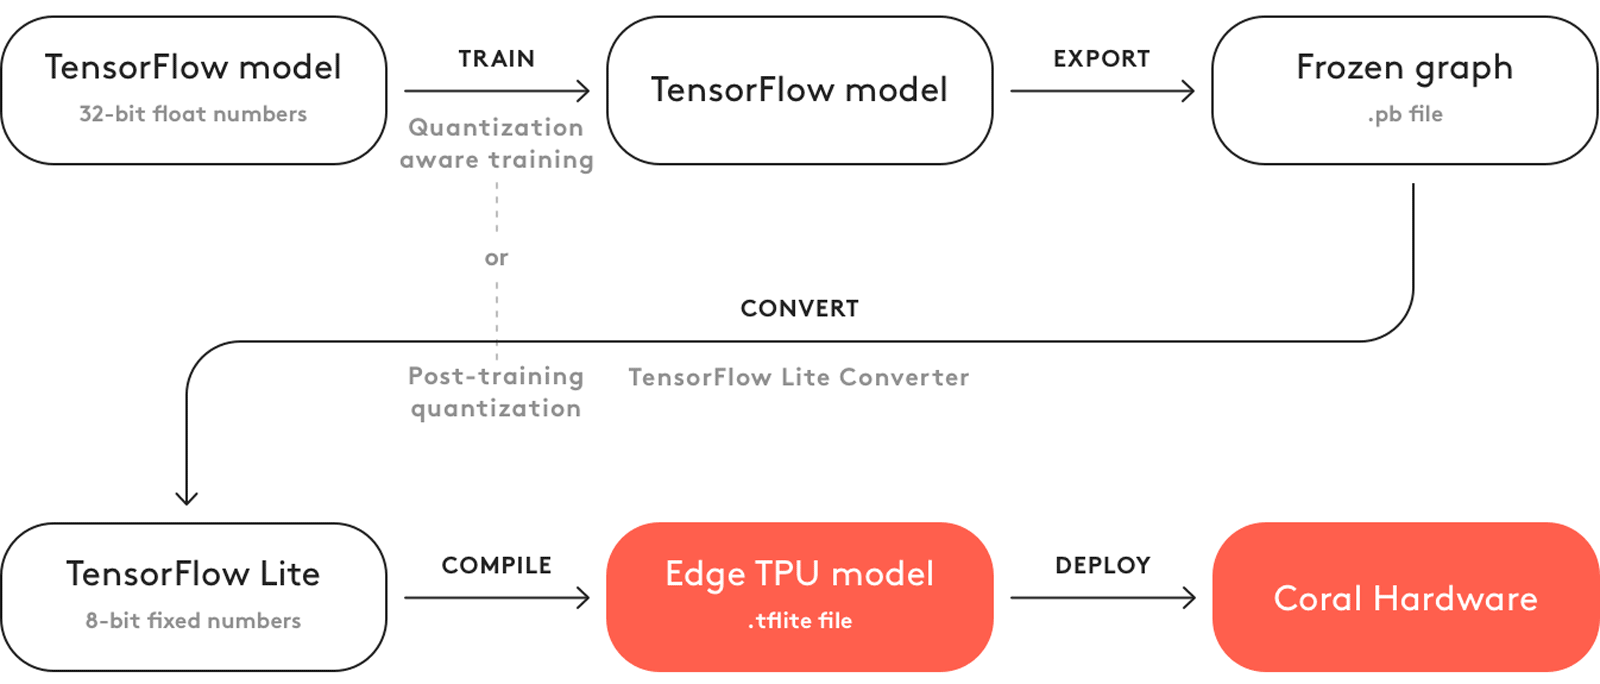
\includegraphics[width=0.95\textwidth]{files/Edge_TPU_quantization.png}
  \caption{The basic workflow to create a model for the \protect\gls{edgetpu}}
  \label{fig:quantization-chart}
\end{figure}

\section{Methodology}

\subsection*{Data}

To efficiently utilize \gls{tf}'s dataset loading and preprocessing capabilities, a versatile data handling method has to be implemented.
A core idea behind this approach is to unify the preparation of training, validation and test subsets within a single configurable function.
This function must manage all aspects of dataset construction and transformation according to user-defined parameters, thereby ensuring consistensy and flexibility.
The function should output \code{tf.data.Dataset}\footnote{\url{https://www.tensorflow.org/api_docs/python/tf/data/Dataset}} objects that are ready for immediate use in training pipelines.

Ideally, the testing pipeline should also be incorporated within this flexible, unified function.
The absence of pre-cropped test subset \gls{gt} patches introduces the necessity for additional preparation steps.

\subsection*{Model}

%Separate from the dataset pipeline, the model architecture is developed independently.
The model architecture is tailored for deployment on embedded systems, where \gls{qat} must be taken into account.
Due to the lack of existing practical examples for deploying this specific model architecture on \gls{edgetpu},
the design process begins with a minimal configuration, using the smallest feasible number of layers and filters,
and gradually increases in complexity based on deployment outcomes and evaluation feedback.
An iterative, trial-and-error methodology is employed, allowing for adjustments in response to the resource constrains encountered on embedded hardware.

The objective is to implement multiple configurable functions, each responsible for constructing a distinct model architecture.
These functions include all necessary helper routines and utilities required to assemble the desired architecture,
allowing convenient switching between models during training.
%These limitations necessitate such architectural decisions, as the use of \gls{qat}.
%For this purpose, model layers are annotaded appropriately to support later quantization and efficient deployment on hardware with limited resources.

\subsection*{Training}
%\label{subsec:designtrain}

After implementing utilities for dataset construction and defining the model architecture, the next step is to develop the training pipeline.
Initially, a simple and direct training pipeline should be created to validate basic model architectures, as a minimal setup both reduces potential error sources and enables rapid proof-of-concept.
During early development, model conversion is performed separately after training.

However, the pipeline should be further refined, ideally as a single executable script, that encompasses data loading, training, configuration management, and model conversion,
streamlining the path to deployment. The goal is to enable a convenient, one-click training and conversion workflow.

To ensure reproducibility and facilitate backups, it is important to store all training configurations, logs, and intermediate model weights for each run.

Finally, computational resources must be considered. To avoid prohibitively long training times, the use of more powerful machines or cloud-based resources should be considered.

\subsection*{Conversion}

After training, the model must be converted and compiled for \gls{edgetpu} inference.
A modular approach is important here as well, simplifying debugging and ensuring correct conversion and compilation during early development.
Later on, the integration of the conversion process directly into the training pipeline is ideal for convenience and efficiency.

Automated use of the \gls{edgetpu} Compiler,
is required so that the entire training and conversion pipeline outputs a model ready for deployment on the \gls{devboard}.

\subsection*{Deployment}
%\label{subsec:designdep}

A tool must be developed on the \gls{devboard}. This program should preload the testing data, load the trained model, and pass
tensors for inference. In early development, for debugging purposes, the testing data can be represented by a single patch.
The goal, however, is scene-wise prediction. Ideally, all necessary steps, from preparing the input data as a series of patches
to stitching the predictions, are implemented in a unified pipeline. The use of C++ inference should be considered for greater control
and potential performance improvements. Inference time must be documented as an important performance metric.

\subsection*{Evaluation}

After successful implementation and verification of the training and deployment pipelines,
multiple versions of \glspl{cnn} can be designed and trained using the developed tools.
Training metrics must be documented. Following successful deployment on the \gls{devboard},
the models will be evaluated on the complete testing dataset.
To minimize the time needed for full-dataset inference, the evaluation is planned to be implemented and executed on a personal workstation.
Models are then evaluated using the metrics outlined in \secshortref{subsec:evalmetrics}.
The results and key insights will be documented for future applications.

}